\documentclass[10pt]{article}


%AMS-TeX packages
\usepackage{amssymb,amsmath,amsthm}

\usepackage{units}

\usepackage{subfigure}

\usepackage[retainorgcmds]{IEEEtrantools}

\usepackage[numbered]{mcode}

% required to get proper length monospace underscores
\usepackage[T1]{fontenc}

%geometry (sets margin) and other useful packages
\usepackage[margin=2.5cm]{geometry}
\usepackage{graphicx,ctable,booktabs}
\begin{document}

\title{Stochastic Optimisation}

\renewcommand{\theenumi}{\alph{enumi}}
\renewcommand{\theenumii}{\arabic{enumii}}
\renewcommand{\labelenumii}{\theenumii.}

% Remove the author field and the space associated with it
% from the definition of maketitle!
\makeatletter
\renewcommand{\@maketitle}{
\newpage
 \null
 \vskip 2em%
 \begin{center}%
  {\LARGE \@title \par}%
    \vskip 1em%
    {\large \@date}%
 \end{center}%
 \par} \makeatother

\maketitle

\thispagestyle{empty}

\section{Introduction}

In this coursework, the problem of global optimisation of Keane's Bump was
solved with Biased Monte Carlo Sampling (BMCS) and with Simulated Annealing
(SA) algorithms. The performance of the algorithms was investigated, as was
the effect of different parameters on the performance.

\section{Problem Description}

\begin{IEEEeqnarray*}{rrCl}
  \textrm{Maximise } & f(\boldsymbol{x}) &=& \left|
    \frac
      {\left(\cos x_1\right)^4 + \left(\cos x_2\right)^4 -
        2\left(\cos x_1\right)^2 \left(\cos x_2\right)^2}
      {\sqrt{x_1^2 + 2 x_2^2}} \right| \\
  \textrm{subject to } & x_1, x_2 &\in& [0, 10] \\
  & x_1 x_2 &>& 0.75 \\
  & x_1 + x_2 &<& 15
  \end{IEEEeqnarray*}

The surface of the feasible region is shown in Figure~\ref{fig:bump_3d}.
Since we can see that the global optimum is on the $x_1 x_2 > 0.75$ boundary,
we can locate it by searching along that curve. This tells us that the optimum
is located at $[1.6009\ 0.4685]^\textrm{T}$, where the objective function is
$0.36498$. There are many other local optima, both on and off the constraint
boundaries.

\begin{figure}
  \begin{center}
    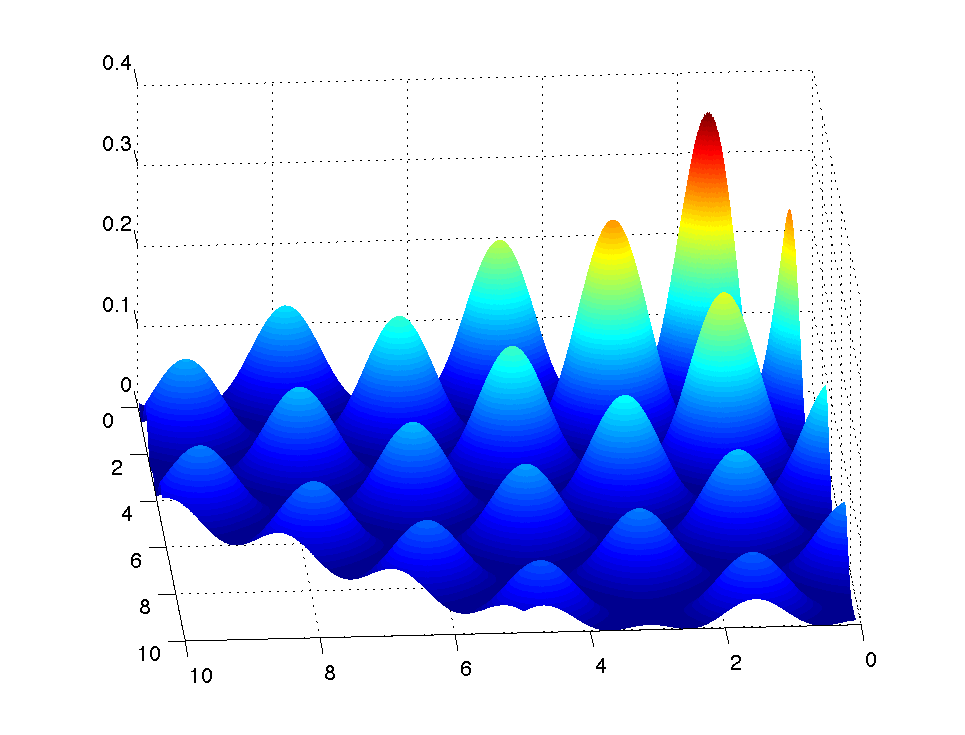
\includegraphics[height=9cm]{bump_3d_smooth.eps}
    \end{center}
    \caption{Keane's 2-D Bump}
    \label{fig:bump_3d}
    \end{figure}

\section{Techniques}

\subsection{Quantifying Performance}

\label{sec:quant_perf}

To investigate the performance of an algorithm with given parameters, it is
run $n$ times with the random seeds $1, 2, \dots, n$, and each time the best
solution found is recorded. To get an impression of the performance, we can
consider the mean $\mu$ and standard deviation $\sigma$ of the results. This
can be likened to approximating the distribution of the results as a Gaussian,
and matching the first and second moments. This approximation can be very bad,
as shown in figure~\ref{fig:result_dist}, but it serves to indicate the
performance of the algorithm. In the cases shown, the Gaussians predict 6\%
and 38\% chances of a result exceeding the global optimum.

\begin{figure}
  \begin{center}
    \mbox{
      \subfigure{
        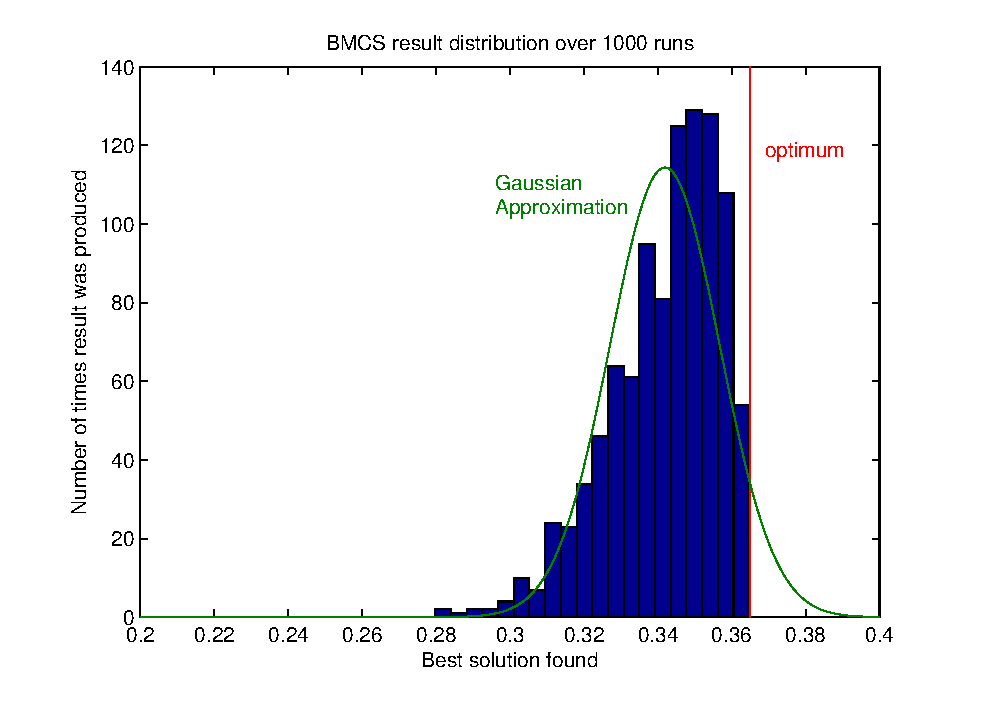
\includegraphics[width=8cm]{bmcs_dist.eps}
      }
      \subfigure{
        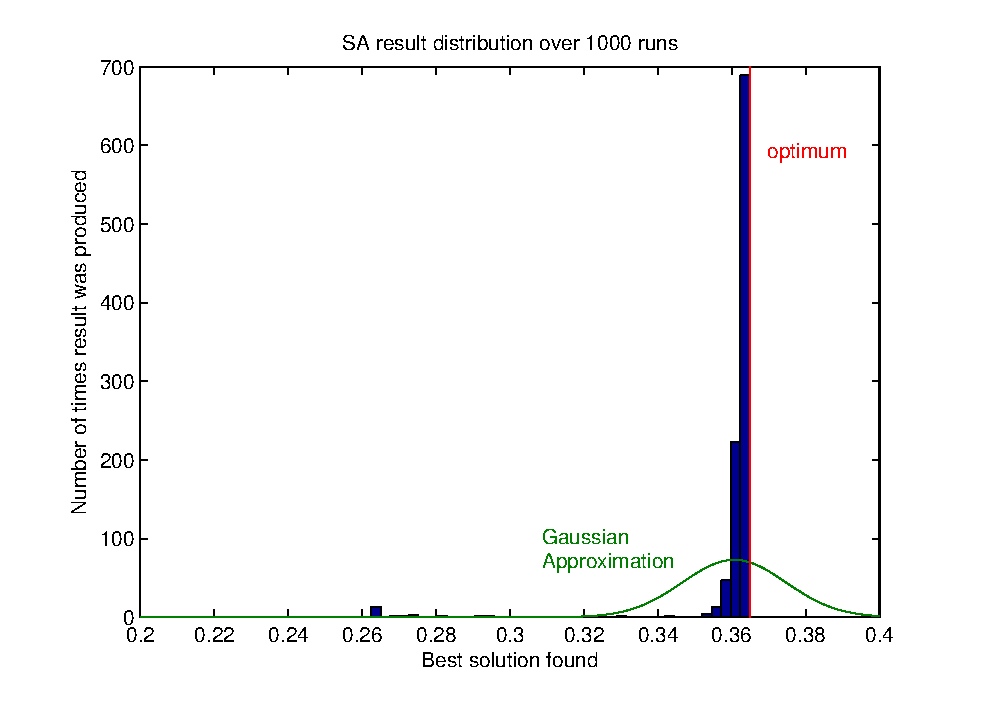
\includegraphics[width=8cm]{sa_dist.eps}
      }
    }
    \end{center}
    \caption{Result distributions and Gaussian approximations}
    \label{fig:result_dist}
    \end{figure}

If we trust the Gaussian approximation, $\mu$ and $\sigma$ are sufficient to
calculate probabilistic bounds for the performance of the algorithm. For
example, in 95\% of cases the result would be above $\mu - 1.645 \sigma$. It
would be more accurate to directly estimate the $5^\textrm{th}$ percentile
from the data and perhaps this should have been used instead. However, one
feature of the Gaussian approach is that it penalises rare, catastrophic
failures heavily.  For the SA results in figure~\ref{fig:result_dist}, the
approximated and actual $5^\textrm{th}$  percentiles are 0.338 and 0.358,
respectively.

Another advantage of calculating the standard deviation is that it can be used
to determine the accuracy of the calculated mean. By the Central Limit
Theorem, as $n \rightarrow \infty$ the distribution of $\mu$ tends to a normal
distribution, $N(\mu_\textrm{true},\ n^{-1}\sigma_\textrm{true}^2)$. Thus,
with a probability of around 95\%,
$\mu_\textrm{true} \in
[\mu-2\,n^{-\nicefrac{1}{2}}\sigma, \mu+2\,n^{-\nicefrac{1}{2}}\sigma]$. This
gives us a statistical confidence bound when we are drawing conclusions about
performance.

Two concerns are ignored in the confidence bound above. Firstly, we assume
$\sigma_\textrm{true} \approx \sigma$---this error will hopefully become
negligible for large n. Secondly, if we are selecting the results with the
highest mean, this will tend to select evaluations with $\mu >
\mu_\textrm{true}$ and will skew the distributions of the estimated $\mu$.

\subsection{Visualising Performance}

\label{sec:vis_perf}

By estimating $\mu$ and $\sigma$ for different parameter settings, we can see
how the parameter settings affect the performance, and we can determine the
parameters that result in the best performance. This is effectively a
multidimensional optimisation of a noisy objective. However, the purpose of
this report is not to find the best parameters for this problem, but to gain
an understanding of how they affect the performance. For this purpose, we need
to be able to see how a single parameter changes the performance, but this is
complicated by the settings of the other
parameters---figure~\ref{fig:bmcs_perf_scatters} shows how complicated this is.  To take
this into account, for a given setting of one parameter we can choose the
other parameters to optimise the performance. This allows us to view the
performance as a function of a single variable, which makes it easier to
visualise and explain.

More formally, given a performance measure $o(\theta_1, \theta_2, \dots,
\theta_k)$, we consider the $k$ different functions:

  \begin{equation*}
    o_i(\theta_i) = \max_{\theta_1 \dots \theta_{i-1}, \theta_{i+1} \dots
    \theta_{k}} o(\theta_1 \dots \theta_k)
    \end{equation*}

\subsection{Penalty Function}

The same penalty function was used in both the BMCS and SA algorithms:
\begin{IEEEeqnarray*}{rCll}
  c(\boldsymbol{x}) &=& \min(x_1 - 0,& 0)\ + \\
  && \min(10 - x_1,& 0)\ + \\
  && \min(x_2 - 0,& 0)\ + \\
  && \min(10 - x_2,& 0)\ + \\
  && \min(15 - x_1 - x_2,\ & 0)\ + \\
  && \min(x_1 x_2 - 0.75,& 0)
  \end{IEEEeqnarray*}

It is scaled by a configurable weight, given by the \mcode{penalty_factor}
variable. In general, we could use separate weights for every constraint, but
since the variable scales are so similar in this problem, this possibility was
not investigated.

\subsection{Archiving}

Archiving was implemented exactly as described in the lecture notes. The same
archiving code was used for the BMCS and SA implementations, and the algorithm
implementations themselves are independent of the number and type of archives
used. One downside of this low-coupling approach is that an implementation
might want to use a dissimilarity archive when restarting the search. This was
avoided by having the SA implementation keep track of the single best solution
seen so far, and restart from there if necessary.

\section{Biased Monte Carlo Sampling}

The BMCS algorithm is much like that shown in lectures. Each axis range is
divided into $m$ equally sized ranges, for a total of $m^2$ regions. To
determine initial region probabilities it samples a certain number of times
per region, then uses the average objective observed in each region to rank
them. The linear selection probability relationship is used to translate the
ranks to probabilities. 1000 random samples are made according to these
probabilities, then the probabilities are recalculated. 

The penalty function is used in two ways: firstly to detect invalid solutions
and to avoid archiving them, and secondly when calculating the average
objective in a region (for determining selection probability).

The following parameters of the algorithm were investigated:

\vspace{5pt}

\begin{tabular}{l | l}
  Parameter & Description \\
  \hline
  \mcode{penalty_factor} & A constant weight used for the penalty function \\
  \mcode{m} & The number of divisions of each axis \\
  \mcode{initial_samples} & The number of samples to take, per region, before
  calculating region probabilities \\
  \mcode{pressure} & The selection pressure, $S$, used when calculating region
  probabilities.
\end{tabular}

\subsection{Searching the Parameter Space}

To investigate the effect of various parameters, the following parameter
values were chosen for investigation:

\vspace{5pt}

\begin{tabular}{l | l l l l l l l l l}
  Parameter & \multicolumn{9}{l}{Values} \\
  \hline
  \mcode{penalty_factor} & 0.01 & 0.1 & 1 & 3 & 10 & 30 \\
  \mcode{m} & 5 & 10 & 15 & 20 & 25 & 30 \\
  \mcode{initial_samples} & 1 & 2 & 3 & 4 & 5 \\
  \mcode{pressure} & 1 & 1.25 & 1.5 & 1.75 & 2 & 3 & 4 & 8 & 16
  \end{tabular}

\vspace{5pt}

The algorithm was run for every combination of these values: a total of 1,620
combinations. For each combination, it was run $n = 1000$ times, as described
in section~\ref{sec:quant_perf}. Figure~\ref{fig:bmcs_perf_scatters} shows the
results.

\begin{figure}
  % thank god LaTeX frees me from worrying about layout!
  \advance\leftskip-1cm
  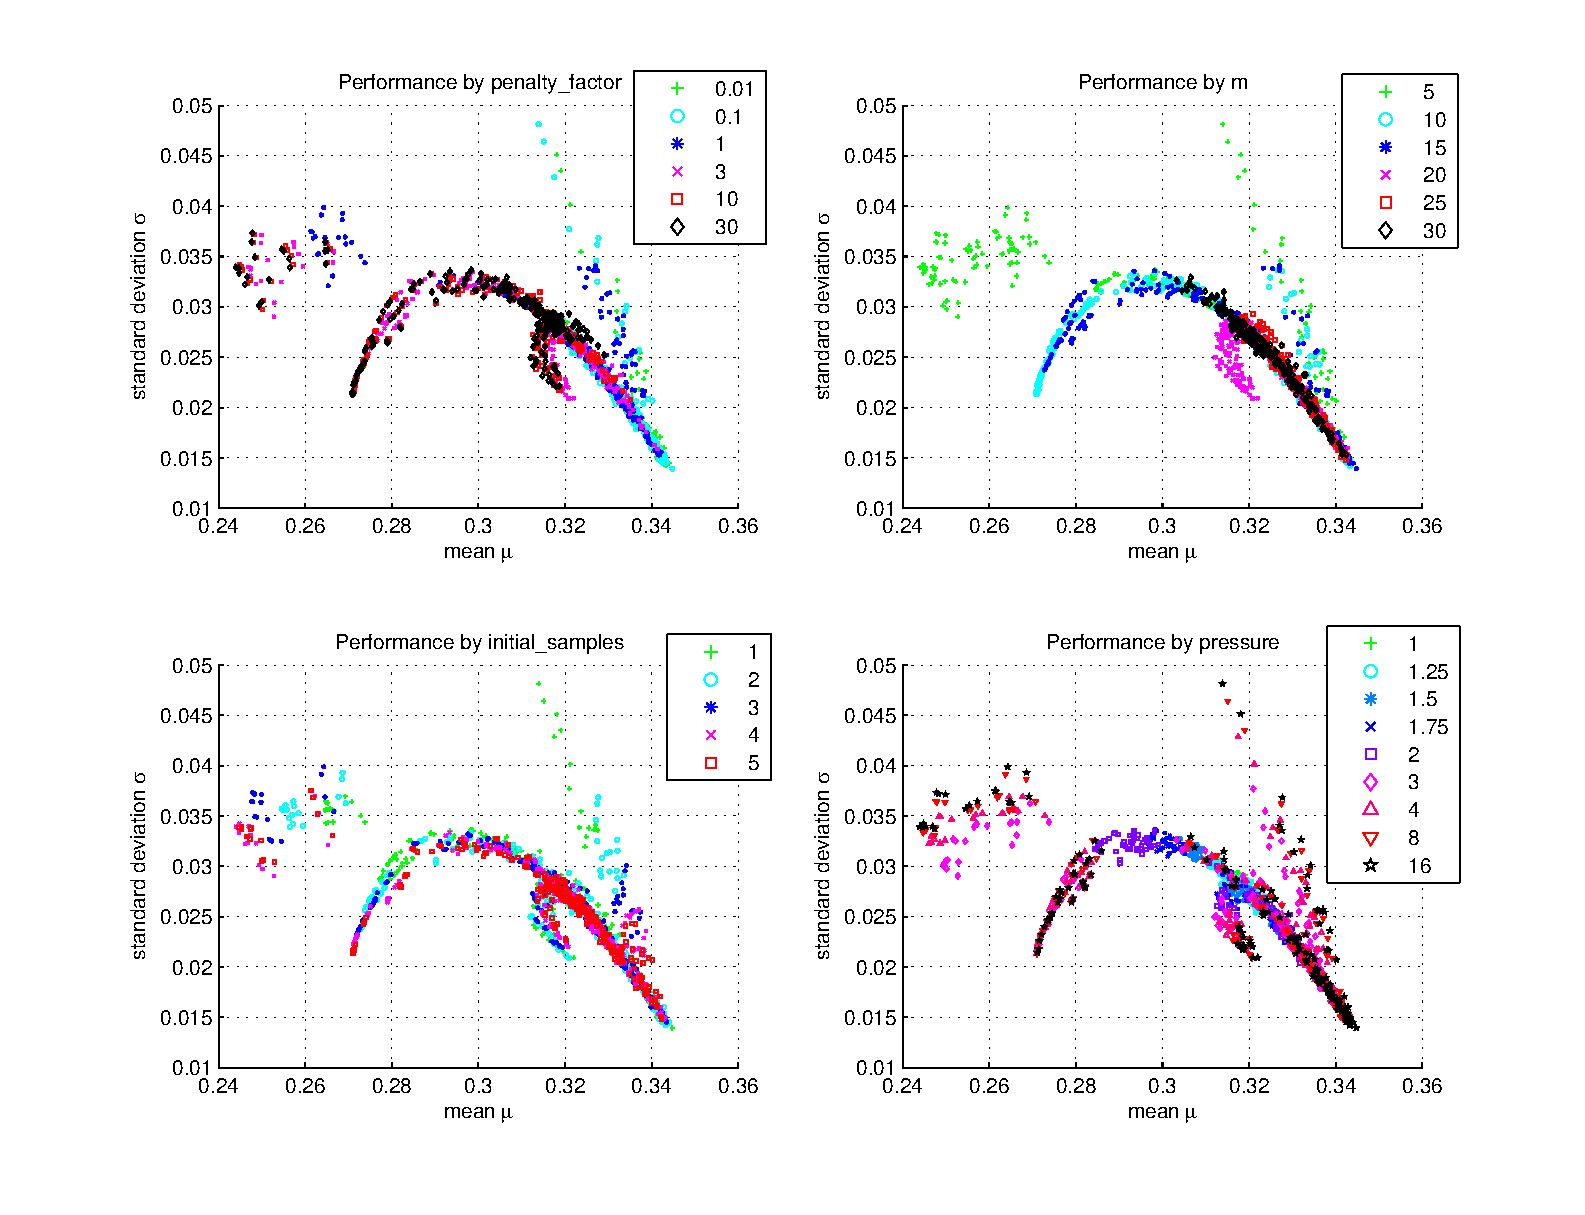
\includegraphics[clip, trim=1.5cm 0.75cm 1.5cm 0.75cm, width=18.5cm]{bmcs_perf_scatters.eps}
  \caption{BMCS performance with varying parameters}
  \label{fig:bmcs_perf_scatters}
  \end{figure}

These plots are rather complicated. They show some striking patterns
(especially the variation with $m$) but it is not clear what is causing these.
Some insights that can be drawn from these plots:

\begin{itemize}
  \item 
    The large bump visible can be explained by analogy to a Bernoulli random
    variable, with $\mu = p$ and $\sigma = \sqrt{p(1-p)}$, where the two values of
    the variable correspond to the two largest optima of the function, peaking at
    0.263 and 0.365.

  \item
    The graph of variation with selection pressure shows that at low pressures
    the performance varies very little when changing other parameters (the
    green and cyan dots are all hidden in the densely packed blob).
    
    At larger selection pressures, (pink, red and black) we start to see
    interesting patterns like the patch on the left, the main curve, curl
    coming off it and the ``jet'' of high variance results above the main
    curve.

  \item
    Similarly, results for smaller regions (larger $m$) are more tightly
    clustered on the graph. In this case, however, the regions can be made
    small without sacrificing performance.

    For larger regions (especially $m = 5$) the performance is very variable,
    and most of the strange features of the graphs are composed of results for
    small $m$.

  \item
    Smaller penalty factors appear to give better performance. However,
    the combination of:
    \begin{itemize}
      \item Small penalty factor
      \item Small m (and thus large regions)
      \item Few initial samples
      \item High selection pressure
    \end{itemize}
    leads to the very high result variances seen in the ``jet''.
    Figure~\ref{fig:bmcs_unreliable} shows why this is: with large regions and
    few initial samples, there is a high probability that the initial samples
    represent the objective function in the region badly---the regions
    contain both optima and zeroes of the function. The high selection
    pressure means that regions with low average objective functions are
    completely ignored, and the search never discovers the optimum in the
    region.

  \begin{figure}
    \begin{center}
      \fbox{
        \subfigure{
          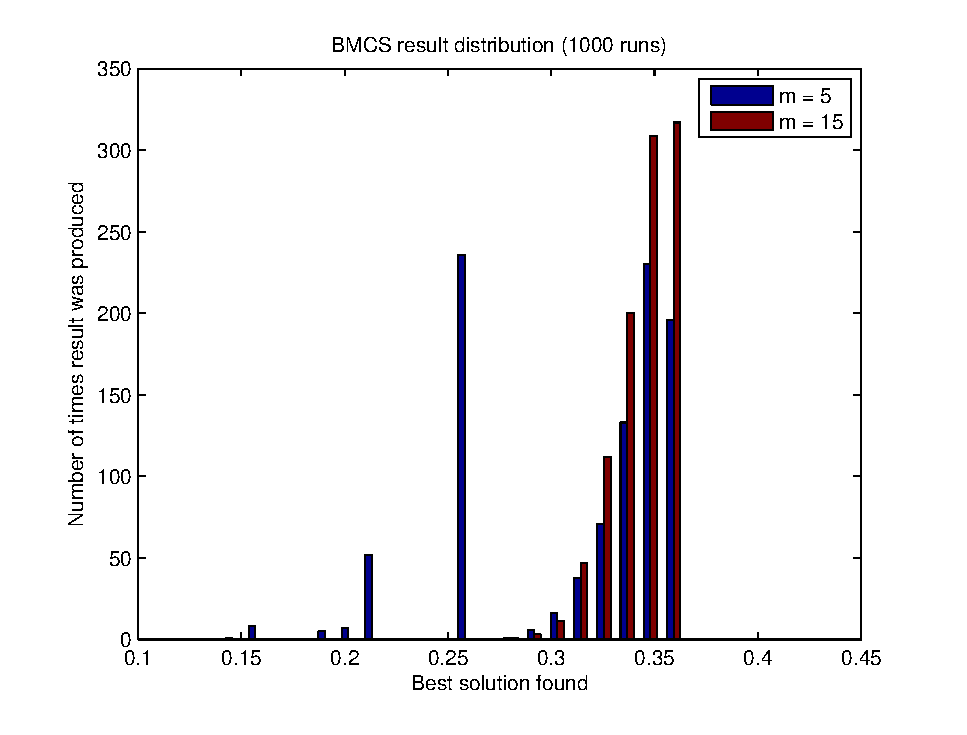
\includegraphics[clip,trim=0.5cm 0cm 0cm 0cm,width=8.5cm]{bmcs_unreliable.eps}
        }
        \subfigure{
          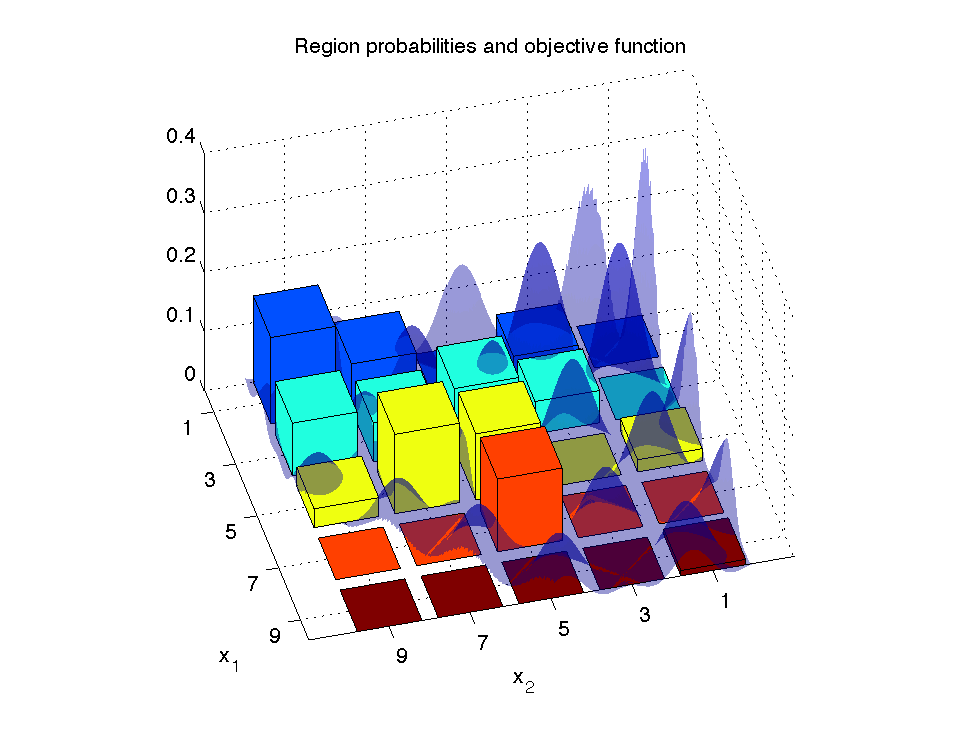
\includegraphics[clip,trim=2cm 0cm 2cm 0cm,width=6.5cm]{bmcs_unreliable_regions.eps}
        }
      }
      \end{center}
      \caption{Small regions leading to an unreliable BMCS}
      \label{fig:bmcs_unreliable}
      \end{figure}

  \item
    Interestingly, when the penalty factor is higher, instead of seeing very
    high variances with high means, we see the lowest means observed but not
    such high variances. This is the patch of results on the left.

    This is because the penalty reduces the chance that sampling will occur
    near the constraints, and concentrates the search on the local optima near
    the centre of the space. Fewer, lower optima lead to a smaller, lower
    range of possible results, and as such smaller $\mu$ and $\sigma$.

\begin{figure}
  \begin{center}
    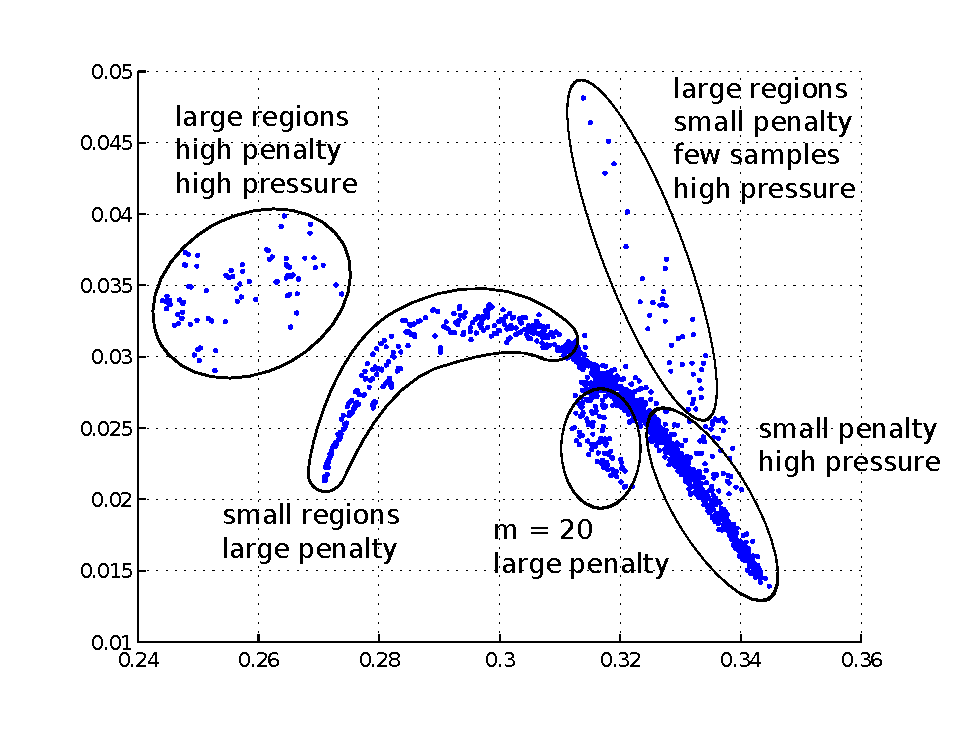
\includegraphics[width=10cm]{bmcs_perf_summary.eps}
    \end{center}
    \caption{Summary of patterns in BMCS performance}
    \label{fig:bmcs_perf_summary}
    \end{figure}

\end{itemize}

\subsection{Effects of Individual Parameters}

\begin{figure}
  \begin{center}
    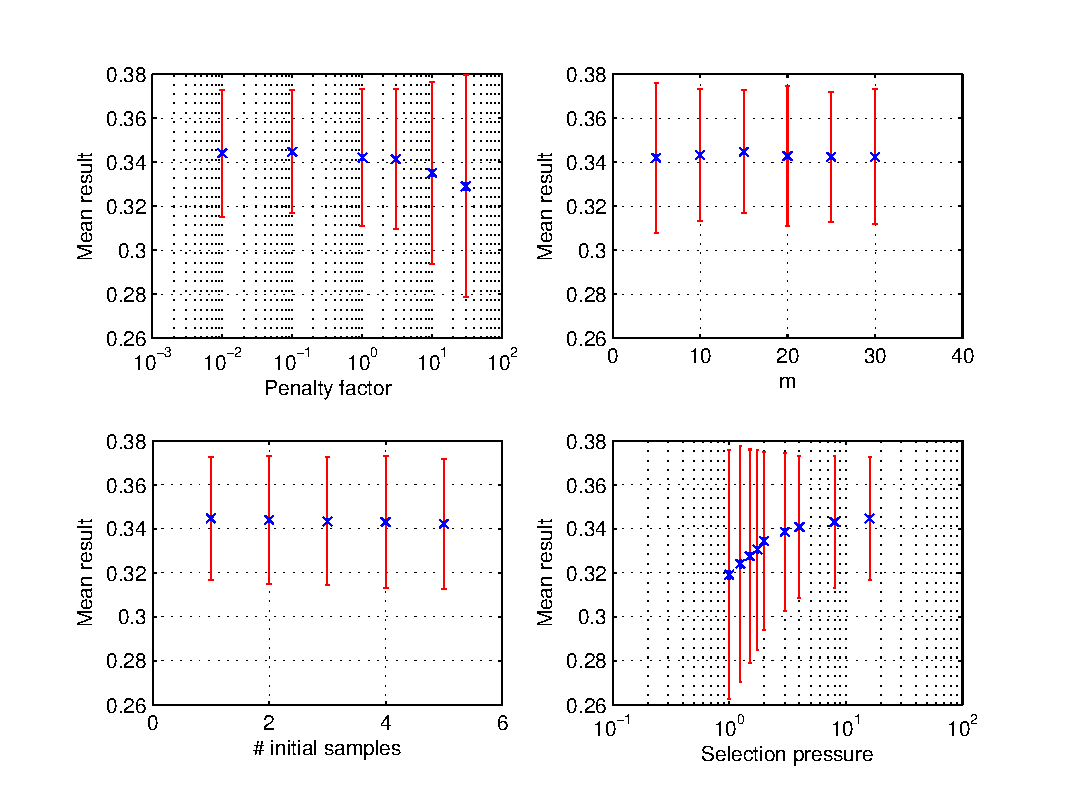
\includegraphics{bmcs_plots.eps}
    \end{center}
    \caption{The effects of constraining individual parameters on best
    performance}
    \label{fig:bmcs_plots}
    \end{figure}

Figure~\ref{fig:bmcs_plots} shows how the performance is affected by
difference parameters. These plots use the method described in
section~\ref{sec:vis_perf}---for each plot, the named parameter is varied and
the others are chosen separately for each point to maximise the mean result.
The blue points are shown with very small blue error bars that indicate the
uncertainty in the estimation of $\mu$. The red error bars stretch $2 \sigma$
in both directions: they are meant to indicate the variability of the
algorithm's performance. Because the result is not normally distributed,
they stretch beyond the maximum possibly result.

\subsection{Summary of BMCS Parameters}

As shown in figures \ref{fig:bmcs_perf_summary} \& \ref{fig:bmcs_plots}, the
parameters that are critical to good performance on this problem are the
penalty weighting factor and the selection pressure. However, appropriate
region sizes and initial samples make the algorithm more robust against
changes in other parameters.

\begin{description}
  \item[Penalty factor] \hfill \\
    If this is much too small, the algorithm may waste time sampling in
    infeasible space. However, if it is too high and the selection pressure is
    high, the algorithm may completely fail to sample optima near constraints.

  \item[Region size] \hfill \\
    If this is much too small (large $m$), the algorithm may waste time in the
    initial survey. If regions are too large, the algorithm becomes very
    sensitive to bad settings of other parameters.
    Figure~\ref{fig:bmcs_perf_scatters} shows how small regions ($m \geq 20$)
    guarantee reasonable performance with the tested parameter ranges.

  \item[Number of initial samples] \hfill \\
    This does not have a particularly great effect on the algorithms
    performance. If the other parameters are set well then just one sample
    per region suffices for good performance, and allows more samples to be
    directed at promising regions. However, setting this $\geq 4$ provides
    protection against the failure shown in figure~\ref{fig:bmcs_unreliable}.

  \item[Selection pressure] \hfill \\
    This plays an important part in making the algorithm efficient.
    Figure~\ref{fig:bmcs_plots} shows that with $S \leq 3$, the algorithm's
    performance is significantly worse, as it doesn't focus its efforts near
    the optima. Setting it very high allows the best performance with
    well-chosen parameters, but causes problems when the regions are too
    small.

\end{description}

The best performing parameter settings tested:

\vspace{5pt}

\begin{tabular}{cccc}
  \
  \mcode{penalty_factor} & 
  \mcode{m} &
  \mcode{initial_samples} &
  \mcode{pressure} \\
  \hline
  0.1 & 15 & 1 & 16 \\
  \end{tabular}<++>

\end{document}
